%==============================================================
%  Surrogate Modeling in Statistical Learning:
%  A Deep Dive into Gaussian Processes
%  GPML Chapters 1 & 2  —  Overleaf-ready Beamer source
%  Author: Prateek Raj  |  IIT Madras  |  June 2026
%==============================================================

\documentclass[aspectratio=169, 10pt,handout]{beamer}

%-------------------------------------------------------------
% THEME & COLOUR SETUP
%-------------------------------------------------------------
\usetheme{Madrid}
\usecolortheme{beaver}

% Custom deep navy + accent palette
\definecolor{iitmblue}{RGB}{10,49,97}       % deep navy (headers)
\definecolor{iitmaccent}{RGB}{180,30,30}    % crimson accent
\definecolor{boxblue}{RGB}{30,60,120}       % tcolorbox title bg
\definecolor{boxbluebg}{RGB}{235,242,255}   % tcolorbox body bg
\definecolor{boxgold}{RGB}{160,120,20}      % example box title
\definecolor{boxgoldbg}{RGB}{252,246,220}   % example box body bg
\definecolor{lightgray}{RGB}{248,248,248}   % slide body bg
\definecolor{mathblue}{RGB}{20,60,140}      % inline math emphasis

% Override Madrid palette
\setbeamercolor{palette primary}  {bg=iitmblue, fg=white}
\setbeamercolor{palette secondary}{bg=iitmblue!80, fg=white}
\setbeamercolor{palette tertiary} {bg=iitmblue!60, fg=white}
\setbeamercolor{palette quaternary}{bg=iitmblue, fg=white}
\setbeamercolor{structure}{fg=iitmblue}
\setbeamercolor{frametitle}{bg=iitmblue, fg=white}
\setbeamercolor{title}{fg=white}
\setbeamercolor{block title}{bg=boxblue, fg=white}
\setbeamercolor{block body}{bg=boxbluebg, fg=black}
\setbeamercolor{block title example}{bg=boxgold, fg=white}
\setbeamercolor{block body example}{bg=boxgoldbg, fg=black}
\setbeamercolor{alerted text}{fg=iitmaccent}
\setbeamercolor{itemize item}{fg=iitmblue}
\setbeamercolor{itemize subitem}{fg=iitmaccent}
\setbeamercolor{enumerate item}{fg=iitmblue}
\setbeamercolor{footline}{bg=iitmblue, fg=white}

% Custom footer with slide numbers on the bottom right (e.g. 3 / 28)
\setbeamertemplate{footline}{%
  \hfill%
  \color{gray!80!black}%
  \scriptsize%
  \insertframenumber\,/\,\inserttotalframenumber\kern1.5em\vskip1.5ex%
}

%-------------------------------------------------------------
% FONTS
%-------------------------------------------------------------
\usepackage[T1]{fontenc}
\usepackage[expansion=false]{microtype}

%-------------------------------------------------------------
% MATH PACKAGES
%-------------------------------------------------------------
\usepackage{amsmath, amssymb, amsthm, bm}
\usepackage{mathtools}
\usepackage{xcolor}

%-------------------------------------------------------------
% LAYOUT / BOXES (tcolorbox)
%-------------------------------------------------------------
\usepackage[most]{tcolorbox}
\tcbuselibrary{skins, breakable}

% ── Blue info box ─────────────────────────────────────────
\newtcolorbox{infobox}[1]{
  enhanced, colback=boxbluebg, colframe=boxblue,
  fonttitle=\bfseries\small, title=#1,
  coltitle=white, attach boxed title to top left={yshift=-2mm, xshift=4mm},
  boxed title style={colback=boxblue, sharp corners},
  sharp corners, boxrule=0.5pt, left=4pt, right=4pt, top=6pt, bottom=4pt
}

% ── Gold example box ──────────────────────────────────────
\newtcolorbox{examplebox}[1]{
  enhanced, colback=boxgoldbg, colframe=boxgold,
  fonttitle=\bfseries\small, title=#1,
  coltitle=white, attach boxed title to top left={yshift=-2mm, xshift=4mm},
  boxed title style={colback=boxgold, sharp corners},
  sharp corners, boxrule=0.5pt, left=4pt, right=4pt, top=6pt, bottom=4pt
}

% ── Two-column equal-split ─────────────────────────────────
\newtcolorbox{leftcol}{
  enhanced, colback=boxbluebg, colframe=boxblue,
  sharp corners, boxrule=0.5pt, left=4pt, right=4pt, top=4pt, bottom=4pt
}
\newtcolorbox{rightcol}{
  enhanced, colback=boxbluebg, colframe=iitmaccent,
  sharp corners, boxrule=0.5pt, left=4pt, right=4pt, top=4pt, bottom=4pt
}

\tcbset{
  rectcard/.style={
    enhanced,
    colback=boxbluebg,
    colframe=boxblue,
    boxrule=0.5pt,
    sharp corners,
    left=4pt,
    right=4pt,
    top=4pt,
    bottom=4pt
  }
}

%-------------------------------------------------------------
% TIKZ (flow chart)
%-------------------------------------------------------------
\usepackage{tikz}
\usetikzlibrary{shapes.geometric, arrows.meta, positioning, fit, calc}

\tikzset{
  flowbox/.style={
    rectangle, rounded corners=4pt,
    minimum width=3.2cm, minimum height=0.75cm,
    text centered, draw=iitmblue, thick,
    fill=boxbluebg, font=\scriptsize\bfseries,
    text width=3.0cm
  },
  flowboxR/.style={flowbox, fill=boxgoldbg, draw=boxgold},
  flowboxG/.style={flowbox, fill=green!8, draw=green!50!black},
  arrow/.style={-Latex, thick, iitmblue},
  arrowR/.style={-Latex, thick, boxgold},
  arrowG/.style={-Latex, thick, green!50!black}
}

%-------------------------------------------------------------
% MISC PACKAGES
%-------------------------------------------------------------
\usepackage{booktabs}
\usepackage{graphicx}
\usepackage{hyperref}
\hypersetup{colorlinks=false, pdfauthor={Prateek Raj}, pdftitle={Surrogate Modeling in Statistical Learning: A Deep Dive into Gaussian Processes}}

%-------------------------------------------------------------
% BEAMER INNER THEME TWEAKS
%-------------------------------------------------------------
\setbeamertemplate{navigation symbols}{}
\setbeamertemplate{itemize item}{\scriptsize\raise1pt\hbox{$\blacktriangleright$}}
\setbeamertemplate{itemize subitem}{\scriptsize\raise1pt\hbox{$\circ$}}
\setbeamerfont{frametitle}{size=\normalsize, series=\bfseries}
\setbeamerfont{block title}{size=\small, series=\bfseries}
\setbeamerfont{block body}{size=\footnotesize}

%-------------------------------------------------------------
% MATH SHORTCUTS
%-------------------------------------------------------------
\newcommand{\GP}{\mathcal{GP}}
\newcommand{\N}{\mathcal{N}}
\newcommand{\R}{\mathbb{R}}
\newcommand{\bw}{\mathbf{w}}
\newcommand{\bx}{\mathbf{x}}
\newcommand{\by}{\mathbf{y}}
\newcommand{\bX}{X}
\newcommand{\bphi}{\boldsymbol{\phi}}
\newcommand{\bmu}{\boldsymbol{\mu}}
\newcommand{\bSigma}{\boldsymbol{\Sigma}}
\newcommand{\btheta}{\boldsymbol{\theta}}
\newcommand{\sn}{\sigma_n^2}
\newcommand{\sigf}{\sigma_f^2}
\newcommand{\Ky}{K_y}
\DeclareMathOperator*{\argmax}{arg\,max}
\DeclareMathOperator*{\argmin}{arg\,min}

%-------------------------------------------------------------
% TITLE PAGE INFORMATION
%-------------------------------------------------------------
\title[GPML Ch.~1 \& 2]{%
  \textbf{Surrogate Modeling in Statistical Learning:}\\[2pt]
  \large A Deep Dive into Gaussian Processes}

\author[Prateek Raj]{%
  \textbf{Prateek Raj (BT23CS021)}}

\institute[IIT Madras]{%
  \footnotesize Indian Institute of Technology Madras\\[4pt]
  \footnotesize Research Intern under the guidance of:\\
  \footnotesize \textbf{Prof.~Neelesh Shankar Upadhye}\\
  \footnotesize Department of Mathematics}

\date{June 2026}

%==============================================================
\begin{document}
%==============================================================

%-------------------------------------------------------------
% SLIDE 1: TITLE
%-------------------------------------------------------------
\begin{frame}[plain]

  \titlepage

\end{frame}

%-------------------------------------------------------------
% SLIDE 2: OUTLINE
%-------------------------------------------------------------
\begin{frame}{Presentation Outline}


  \vspace{-2pt}
  
  \begin{columns}[t]
    \column{0.48\textwidth}
      
      \begin{block}{1.\ Introduction \& Inductive Bias}
        \scriptsize
        
        \begin{itemize}\setlength\itemsep{0pt}
          \item Supervised Learning Setup
          \item The Inductive Ambiguity Problem
          \item Restriction Bias vs.\ Preference Bias
          \item Bayes' Rule \& Weight Priors
        \end{itemize}
      \end{block}
      

      \begin{block}{2.\ Gaussian Process Regression}
        \scriptsize
       
        \begin{itemize}\setlength\itemsep{0pt}
          \item Weight-Space Bayesian Linear Regression
          \item Feature Space \& Dimension Bottleneck
          \item Kernel Trick \& Function-Space View
          \item Hyperparameter Tuning \& Occam's Razor
          
        \end{itemize}
      \end{block}
      
      

  \end{columns}

\end{frame}

%==============================================================
%  PART 1 — CHAPTER 1: INTRODUCTION & INDUCTIVE BIAS
%==============================================================

%-------------------------------------------------------------
% SLIDE 3: SUPERVISED LEARNING SETUP
%-------------------------------------------------------------
\begin{frame}{Supervised Learning Setup}


  \begin{itemize}
    \item \textbf{Definition:} Given training examples of inputs (X) and
      corresponding outputs (Y), find the underlying relationship:
      \[
        y = f(\bx)
      \]
      
    \item \textbf{Generalisation:} For a new input $\bx_*$, predicting the
      corresponding target $y_*$ is called generalisation $(f:X\to Y)$.
      
    \item \textbf{Problem Types:}
      \begin{itemize}
        \item \textbf{Regression:} Output target is a continuous numerical value
          (e.g., age, house price, temperature).
        \item \textbf{Classification:} Output target belongs to a discrete
          category (e.g., cat/dog, pass/fail).
      \end{itemize}
    
  \end{itemize}

\end{frame}

%-------------------------------------------------------------
% SLIDE 4: INDUCTIVE BIAS — CORE PROBLEM
%-------------------------------------------------------------
\begin{frame}{The Core Problem: Inductive Bias}

  \begin{itemize}
    \item \textbf{Under-determination Problem:}  The training data alone cannot
      uniquely identify the true function.  There are infinitely many functions
      that satisfy the dataset. 
  \end{itemize}
  \vspace{4pt}
  \begin{examplebox}{Example — Ambiguity in Curve Fitting}
    \vspace{8pt}
    \begin{columns}[T]
      \column{0.44\textwidth}
        \scriptsize
        Given points $(1,0)$, $(2,0)$, $(3,0)$, possible functions include:
        \begin{align*}
          f_1(x) &= (x-1)(x-2)(x-3)\\
          f_2(x) &= (x-1)(x-2)(x-3) + \sin(x-1)\sin(x-2)\sin(x-3)
        \end{align*}
      \column{0.26\textwidth}
        \centering
        \textbf{\tiny Curve 1 ($f_1$)}\\
        \vspace{2pt}
        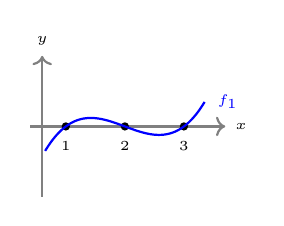
\begin{tikzpicture}[x=0.75cm, y=0.28cm]
          % Draw axes
          \draw[->, thick, gray] (0.4,0) -- (3.7,0) node[right, black] {\tiny $x$};
          \draw[->, thick, gray] (0.6,-3.2) -- (0.6,3.2) node[above, black] {\tiny $y$};
          
          % Draw labels on x-axis
          \foreach \x in {1,2,3} {
            \draw (\x,0.12) -- (\x,-0.12);
            \node[below=2pt] at (\x,0) {\tiny \x};
            \fill[black] (\x,0) circle (1.5pt);
          }
          
          % Draw f1 (blue line)
          \draw[domain=0.65:3.35, samples=60, smooth, thick, blue] 
            plot (\x, {(\x-1)*(\x-2)*(\x-3)}) node[right=1pt] {\tiny $f_1$};
        \end{tikzpicture}
      \column{0.26\textwidth}
        \centering
        \textbf{\tiny Curve 2 ($f_2$)}\\
        \vspace{2pt}
        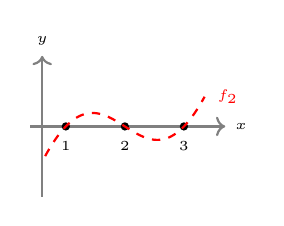
\begin{tikzpicture}[x=0.75cm, y=0.28cm]
          % Draw axes
          \draw[->, thick, gray] (0.4,0) -- (3.7,0) node[right, black] {\tiny $x$};
          \draw[->, thick, gray] (0.6,-3.2) -- (0.6,3.2) node[above, black] {\tiny $y$};
          
          % Draw labels on x-axis
          \foreach \x in {1,2,3} {
            \draw (\x,0.12) -- (\x,-0.12);
            \node[below=2pt] at (\x,0) {\tiny \x};
            \fill[black] (\x,0) circle (1.5pt);
          }
          
          % Draw f2 (red dashed line)
          \draw[domain=0.65:3.35, samples=100, smooth, thick, red, dashed] 
            plot (\x, {(\x-1)*(\x-2)*(\x-3) + sin((\x-1)*57.2958)*sin((\x-2)*57.2958)*sin((\x-3)*57.2958)}) node[right=1pt] {\tiny $f_2$};
        \end{tikzpicture}
    \end{columns}
  \end{examplebox}
  
  

  \vspace{4pt}
  \begin{itemize}
    \item \textbf{Inductive Bias:} The set of additional assumptions we impose
      on the learning algorithm to prefer a specific function over others.
    \item \textit{Every machine learning algorithm contains some form of
      inductive bias.}
  \end{itemize}

\end{frame}

%-------------------------------------------------------------
% SLIDE 5: RESTRICTION BIAS vs PREFERENCE BIAS
%-------------------------------------------------------------
\begin{frame}{The Fork: How We Enforce Our Assumptions} 

  How do we actually impose this bias in our learning algorithm?
  There are two main strategies:

  \vspace{8pt}
  
  \begin{columns}[t]
    \column{0.48\textwidth}
      
      \begin{block}{1.\ Restriction Bias}
        Restrict the set of allowed functions.
        Confine the search space to a rigid,
        parameterized family of curves.

        \medskip
        \textbf{Model Type:} Parametric Models
        (e.g., Linear functions).
      \end{block}
      

    \column{0.48\textwidth}
      \begin{block}{2.\ Preference Bias}
        Allow a very large (or infinite) class
        of functions, but place a probability
        distribution over them, preferring some
        over others.

        \medskip
        \textbf{Model Type:} Non-Parametric
        Bayesian Models (e.g., GPs).
      \end{block}
  \end{columns}

\end{frame}

%-------------------------------------------------------------
% SLIDE 6: RESTRICTION BIAS + NOISE MODEL
%-------------------------------------------------------------
\begin{frame}{Restriction Bias: The Parametric View} 

  \begin{itemize}
    \item \textbf{Parametric Model:} Look for a solution within a specific
      family determined by a \emph{finite} number of parameters $\bw$.
    \item \textbf{Simple Linear Model:}
      \[
        f(\bx) = \bx^T\bw,
        \quad
        \bx=[x_1,\dots,x_d]^T,\;
        \bw=[w_1,\dots,w_d]^T
      \] 
    \item \textbf{Drawback:}  The model is strictly prohibited from considering
      non-linear curves, oscillatory functions, or complex local gradients,
      leading to under-fitting.
  \end{itemize}
  

  \vspace{4pt}
  \begin{block}{Measurement Noise}
    The models  are never perfect.  We model this by adding noise
    $\epsilon$:
    \[
      y = f(\bx) + \epsilon
    \]
  \end{block}

\end{frame}

%-------------------------------------------------------------
% SLIDE 7: GAUSSIAN NOISE & LIKELIHOOD
%-------------------------------------------------------------
\begin{frame}{Real Data Noise \& Likelihood}

  \begin{columns}[T]
    \column{0.48\textwidth}
      \begin{block}{Why Gaussian Noise?}
        \scriptsize
        \begin{itemize}
          \item \textbf{Central Limit Theorem:} Sum of many natural random errors approximately converges to a Gaussian.
            \begin{itemize}
              \item \tiny \textbf{Ref:} Jaynes, E. T. (2003). \emph{Probability Theory: The Logic of Science}. Cambridge University Press.
            \end{itemize}
          \item \textbf{Analytical Convenience:} Easy to manipulate mathematically, yielding closed-form solutions.
        \end{itemize}
      \end{block}

    \column{0.48\textwidth}
      
      \begin{block}{Noise Model}
        \scriptsize
        We assume i.i.d. additive Gaussian noise:
        \[
          \epsilon_i \sim \N(0, \sigma_n^2), \quad y_i = f(\bx_i) + \epsilon_i
        \]
      \end{block}
      

      \begin{block}{The Likelihood Function}
        \scriptsize
        \textbf{Single Datapoint $(\bx_i, y_i)$:}
        \[
          p(y_i \mid \bx_i, \bw) = \N(\bx_i^T\bw, \, \sigma_n^2)
        \]
        \textbf{Entire Dataset $(X, Y)$:}
        \[
          p(Y \mid X, \bw) = \N(X\bw, \, \sigma_n^2 I)
        \]
      \end{block}
  \end{columns}

  \vspace{4pt}
  \begin{block}{Term Notation}
    \scriptsize
    \begin{tabular}{ll}
      $\bx_i \in \mathbb{R}^d$ : Input vector for point $i$ & 
      $y_i \in \mathbb{R}$ : Target output for point $i$ \\
      $X = [\bx_1, \dots, \bx_n]^T \in \mathbb{R}^{n \times d}$ : Design matrix & 
      $Y = [y_1, \dots, y_n]^T \in \mathbb{R}^n$ : Target vector \\
      $\bw \in \mathbb{R}^d$ : Model weights vector & 
      $\sigma_n^2$ : Noise variance ($I$ is the identity matrix)
    \end{tabular}
  \end{block}

\end{frame}

%-------------------------------------------------------------
% SLIDE 8: BAYESIAN VIEW / BAYES' RULE
%-------------------------------------------------------------
\begin{frame}{Preference Bias: The Bayesian View}

  Instead of excluding non-linear functions (restriction), we adopt a flexible
  Bayesian approach:
  \begin{itemize}
    \item All functions are allowed, but we assign probabilities to them
      (e.g., simple functions are more likely; highly complex ones are less likely).
    \item \textbf{Bayes' Rule:}
      \[
        P(\bw\mid D) = \frac{P(D\mid\bw)\,P(\bw)}{P(D)}
      \]
  \end{itemize}

  \vspace{4pt}
  
  \begin{columns}[T]
    \column{0.31\textwidth}
      
      \begin{block}{Posterior $P(\bw\mid D)$}
        Belief about weight parameters \emph{after} observing data.
      \end{block}
    \column{0.31\textwidth}
      \begin{block}{Prior $P(\bw)$}
        Initial belief \emph{before} seeing data.  This is where
        \textbf{inductive bias} enters.
      \end{block}
    \column{0.31\textwidth}
      \begin{block}{Evidence $P(D)$}
        Normalizing constant (marginal likelihood).
      \end{block}
  \end{columns}

\end{frame}

%-------------------------------------------------------------
% SLIDE 9: PRIOR OVER WEIGHTS
%-------------------------------------------------------------
\begin{frame}{Prior over Weights}

  \begin{itemize}
    \item We place a zero-mean Gaussian prior on the weight vector:
      \[
        \bw \sim \N(\mathbf{0},\,\bSigma_p)
      \] 
    \item \textbf{Prior Mean $= \mathbf{0}$:} Reflects our expectation that
      smaller weights are more likely. Positive and negative weights cancel
      out.
    \item \textbf{Prior Covariance $\bSigma_p$:} Determines the dispersion of weights around the prior mean $\mathbf{0}$ (diagonal elements) and the Measures, how two weight vary together (off-diagonal elements).
  \end{itemize} 

  \vspace{4pt}
  \begin{block}{Combining Prior and Likelihood}
    Multiplying the likelihood and the prior is proportional to \textbf{posterior
    distribution} over the weights, which is the key object in Bayesian
    Linear Regression.
  \end{block}

\end{frame}

%==============================================================
%  PART 2 — CHAPTER 2: GAUSSIAN PROCESS REGRESSION
%==============================================================

%-------------------------------------------------------------
% SLIDE 10: WEIGHT-SPACE VIEW (THE MERGE)
%-------------------------------------------------------------
\begin{frame}{The Merge: Weight-Space View}

  \begin{itemize}
    \item \textbf{Weight-Space View:} The function is expressed in terms of the
      weight vector $\bw$.  Instead of finding a single best weight vector,
      we maintain a \emph{probability distribution} over all possible weights.
    \item \textbf{Conjugate Property:} Since both the prior and likelihood are
      Gaussian, the posterior is also Gaussian:
      \[
        p(\bw\mid X, Y)=\N(\bmu_{\text{post}},\,\bSigma_{\text{post}})
      \]
    \item \textbf{Completing the Square:} We expand the exponent of $p(Y\mid X,\bw)p(\bw)$ and match its quadratic and linear weight terms to the standard Gaussian exponent $-\frac{1}{2}(\bw-\bmu)^T\bSigma^{-1}(\bw-\bmu)$:
      \begin{itemize}
        \item \textbf{Quadratic term matching:} $\bSigma_{\text{post}}^{-1} = \bSigma_p^{-1} + \frac{1}{\sigma_n^2}X^TX$
        \item \textbf{Linear term matching:} $\bSigma_{\text{post}}^{-1}\bmu_{\text{post}} = \frac{1}{\sigma_n^2}X^T Y$
      \end{itemize}
      \[
        \bSigma_{\text{post}} = \left(\bSigma_p^{-1}+\tfrac{1}{\sn}X^TX\right)^{-1},
        \quad
        \bmu_{\text{post}} = \bSigma_{\text{post}}\tfrac{1}{\sn}X^T Y
      \]
  \end{itemize}

\end{frame}

%-------------------------------------------------------------
% SLIDE 11: PREDICTIVE DISTRIBUTION (WEIGHT-SPACE)
%-------------------------------------------------------------
\begin{frame}{Predictive Distribution in Weight-Space}

  \begin{itemize}
    \item \textbf{Classical Regression:} Chooses one weight vector $\bw$ and
      predicts $y_*=\bx_*^T\bw$, providing no estimation of uncertainty.
    \item \textbf{Bayesian Regression:} Averages predictions over all possible
      weights, weighted by their posterior probabilities:
      \[
        p(y_*\mid\bx_*,\mathcal{D})
          = \int p(y_*\mid\bx_*,\bw)\,p(\bw\mid X, Y)\,d\bw
      \]
    \item Evaluating this integral yields:
      \[
        y_*\mid\bx_*,\mathcal{D}
          \;\sim\;
          \N\!\left(
            \tfrac{1}{\sn}\bx_*^T\bSigma_{\text{post}}X^T Y,\;
            \bx_*^T\bSigma_{\text{post}}\bx_*
          \right)
      \]
    \item This gives both the \textbf{predictive mean} (our estimate) and
      \textbf{predictive variance} (our uncertainty).
  \end{itemize}

\end{frame}

%-------------------------------------------------------------
% SLIDE 12: FEATURE PROJECTIONS
%-------------------------------------------------------------
\begin{frame}{Feature Projections}

  \begin{itemize}
    \item Since real-world relationships are rarely linear, we transform the
      input vector $\bx \in X$ into a high-dimensional feature space using basis
      functions $\phi(\bx)$:
      \[
        f(\bx) = \phi(\bx)^T\bw
      \]
    \item The model remains \emph{linear} in terms of weights $\bw$, but is
      now highly \emph{non-linear} in terms of input $\bx$.
  \end{itemize}

  \vspace{4pt}
  \begin{examplebox}{Polynomial Projection --- For a scalar input $x$:}
    \[
      \phi(x) = \bigl(1,\,x,\,x^2,\,x^3,\,\dots\bigr)^T
    \]
    Any degree polynomial fit becomes a \emph{linear} model in this
    feature space.
  \end{examplebox}

\end{frame}

%-------------------------------------------------------------
% SLIDE 13: DIMENSION BOTTLENECK
%-------------------------------------------------------------
\begin{frame}{The Dimension Bottleneck}

  \begin{columns}[T]
    \column{0.44\textwidth}
      \begin{block}{The Bottleneck ($N \times N$)}
        \footnotesize
        If the feature space has dimension $N$ (where $N$ is very large), calculating the posterior covariance is computationally impossible:
        \[
          \bSigma_{\text{post}} = \left(\bSigma_p^{-1}+\tfrac{1}{\sn}\Phi^T\Phi\right)^{-1}
        \]
        This is the \alert{\textbf{Dimension Bottleneck}} of size $N\times N$.
      \end{block}

    \column{0.52\textwidth}
      \begin{block}{The Woodbury Solution ($n \times n$)}
        \scriptsize
        Applying the Woodbury identity:
        \[
          (B + U C V)^{-1} = B^{-1} - B^{-1} U (C^{-1} + V B^{-1} U)^{-1} V B^{-1}
        \]
        Selecting:
        \[
          B = \bSigma_p^{-1}, \quad U = \Phi^T, \quad C = \sigma_n^{-2} I, \quad V = \Phi
        \]
        Rewritten formula as a result:
        \[
          \bSigma_{\text{post}} = \bSigma_p - \bSigma_p\Phi^T\left(\Phi\bSigma_p\Phi^T + \sn I\right)^{-1}\Phi\bSigma_p
        \]
        This allows us to invert a matrix of size $n\times n$ (data points) instead of $N\times N$ (features).
      \end{block}
  \end{columns}

\end{frame}


\end{document}

